\documentclass[12pt]{article}
\pagestyle{headings}
\setlength{\textheight}{8.67in}
\setlength{\textwidth}{5.8in}
\setlength{\topmargin}{-3mm}
\setlength{\headsep}{40pt}
\setlength{\evensidemargin}{-3mm}
\setlength{\parskip}{.05in}
\setlength{\parindent}{3ex}
\renewcommand{\baselinestretch}{1.2}
\usepackage{amsthm}
\usepackage{graphicx}
\setlength{\headsep}{40pt}
\usepackage{graphicx}
\usepackage{color}
\usepackage{array}
\usepackage{amsmath,amssymb}
\usepackage{epstopdf}
\usepackage{tikz}
\setlength{\topmargin}{-3mm}
\setlength{\leftmargin}{.1in}
\setlength{\footskip}{0.5in}
\pagestyle{myheadings}
\pagenumbering{arabic}
\theoremstyle{definition}
\setlength{\unitlength}{1cm}
\thicklines
\begin{document}
		\section{Matrix Representation of Linear Transformation}
	
	Let $ T:V\to V $ and $ \mathfrak{B} =\{u_{1},u_{2},...,u_{n}\} $ be the basis for the set V.\\
	If $f(t)$ is a polinomial in $\mathbb{F}$ and $T$ is represented by a diagonal matrix . 
	$
	\Lambda =
	\begin{bmatrix}
	\lambda_{1} & 0 &... & 0 \\
	0 & \lambda_2 & ... & 0 \\
	0 & 0 & ... & 0 \\
	0 & 0 & ... &  \lambda_n  \\
	\end{bmatrix}
	$
	\\
	then $P(T)$ is presented with respect to the same basis by 
	$
	P_{\lambda}
	\begin{bmatrix}
	P_{\lambda_{1}} & 0 &... & 0 \\
	0 & P_{\lambda_2} & ... & 0 \\
	0 & 0 & ... & 0 \\
	0 & 0 & ... &  P_{\lambda_n}  \\
	\end{bmatrix}
	$
	When $T \in L(V)$, does there exist an ordered basis for $V$ with respect to $T$ so that $T$ has a diagonal representation?If such a diagonal representation exists,how to find the ordered basis?\\
	\begin{center}
		\begin{picture}(7,7)
		%\put(0,0){0,0}\put(8,0){8,0}\put(0,8){0,8}\put(8,8){8,8}
		\put(2,2){\circle{4}}\put(6,2){\circle{4}}\put(2,6){\circle{4}}\put(6,6){\circle{4}}
		\qbezier(2,6)(4,7)(6,6)\put(4,6.5){\vector(1,0){0.2}}
		\qbezier(2,2)(4,1.4)(6,2)\put(4,1.689){\vector(1,0){0.2}}
		\qbezier(2,6)(1,4)(2,2)\put(1.5,4){\vector(0,1){0.2}}
		\qbezier(6,6)(5,4)(6,2)\put(5.5,4){\vector(0,1){0.2}}
		\put(4,6.7){$ \Lambda $}\put(1.1,4){$ \phi $}\put(5.1,4){$ \phi $}\put(4,1.3){$ T$}
		\put(1.6,1.8){$ u_{i} $}\put(2.1,2.1){$ \mathbb{V} $}
		\put(5.8,1.6){$Tu_{i} $}\put(6.1,2.1){$ \mathbb{V} $}
		\put(1.6,5.9){$ e_{i} $}\put(1.9,6.3){$ \mathbb{F}^{n} $}
		\put(6,5.9){$ \lambda_{i} e_{i} $}\put(5.65,6.3){$ \mathbb{F}^{n} $}
		\end{picture}
	\end{center}
$ \Lambda $ maps $ \mathbb{F}^{n} $ to $ \mathbb{F}^{n} $ and has the property that $$\Lambda e_{i}=\lambda e_{i} $$ $$T( u_{i})=\lambda e_{i} $$ where $ u_{i}=\phi^{-1}(e_{i}) $, ($ i=1,2,3,...n $)\\$ \implies \lambda_{1}, \lambda_{2} ,...\lambda_{n} $ are the eigen values of $ T $ and $ u_{1},u_{2},...,u_{n} $ are the corresponding eigen vectors. \\$$ Tu_{i}=\lambda_{i}u_{i} $$ $ \hspace*{5.5cm} T(\phi^{-1}e_{i})=\lambda_{i}\phi^{-1}e_{i} $\\$ \hspace*{4.9cm} (\phi T \phi^{-1})(e_{i})=\Lambda e_{i}=\lambda_{i}e_{i}=\lambda_{i}\phi(u_{i}) $\\ $ \hspace*{4.6cm} \phi^{-1}\phi T(\phi^{-1}e_{i})=\phi^{-1}\lambda_{i}\phi (u_{i}) $\\$ \hspace*{5.5cm} T(\phi^{-1}e_{i})=\lambda_{i}\phi^{-1}e_{i}
$\\$ \hspace*{5.3cm} T(\phi^{-1}(e_{i}))=\lambda_{i}u_{i} $\\$\hspace*{6.5cm} Tu_{i}=\lambda_{i}u_{i} $\\
So the problem reduces to finding $u_{i}$'s which are eigen vectors of $ T $ such that $ \{u_{1},u_{2},...,u_{n}\} $ forms an ordered basis for $ \mathbb{V} $. It is not always possible.
\begin{center}
\begin{tikzpicture}
\draw (2,2) circle (2cm);
%\draw[step=1cm,gray,very thin] (0,0) grid (4,4);
\qbezier(0,2)(2,2.5)(2,0)\qbezier(1,2)(2,3)(1,3.7)
\qbezier(1.5,3)(2,2.5)(3.7,3)\qbezier(3.8,1)(3,2)(1.9,1)
\put(2,2){$ M^{nxn}(\mathbb{F}) $}
\end{tikzpicture}
\end{center}
\end{document}	